\textbf{Did the bias values converge at the end? What values did they converge to?}\\

The accelerometer bias was calculated as part of our EKF implementation. The bias was the last 3 variables in our state vector ($b_x$, $b_y$, $b_z$). The implementation of the EKF allows the accelerometer bias to be calculated through the following steps:\\

1. Accelerometer bias is included in the state vector\\
2. The IMU data is used to predict the state estimates and it helps propagate the bias\\
3. The state estimate is corrected in the update step of EKF using GPS and accelerometer data, and this in turn also updates the bias\\
4. The EKF estimated bias will be updated through adjustments made between the difference in the actual and predicted measurements, taking into account drift or change in bias over time.\\

As Figure (8) below shows, the accelerometer bias values did converge at the end. The $b_x$ converged to 0.165 $m/s^2$, the $b_y$ converged to -0.252 $m/s^2$, and the $b_z$ converged to -0.087 $m/s^2$. The code to obtain the graph can be seen in Figure (7).

\begin{minipage}[H]{0.43\textwidth}
    \centering    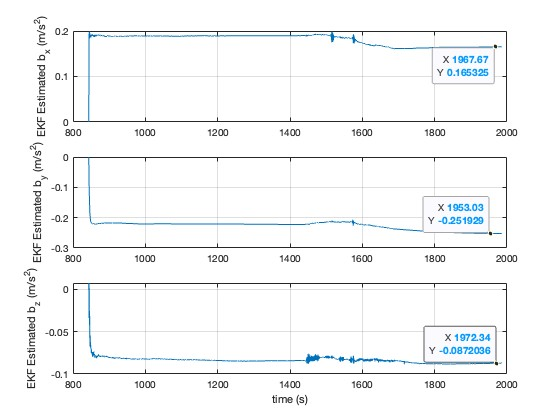
\includegraphics[width=1.6\linewidth]{EKF/EKF_Acb.jpg}  
    \label{fig:EKFAcb}
    \captionsetup{justification=centering} % Ensure caption is centered
    \captionof{figure}{EKF Estimated Accelerometer Bias}
\end{minipage}
\hfill
\begin{minipage}{0.2\textwidth}
    \centering
    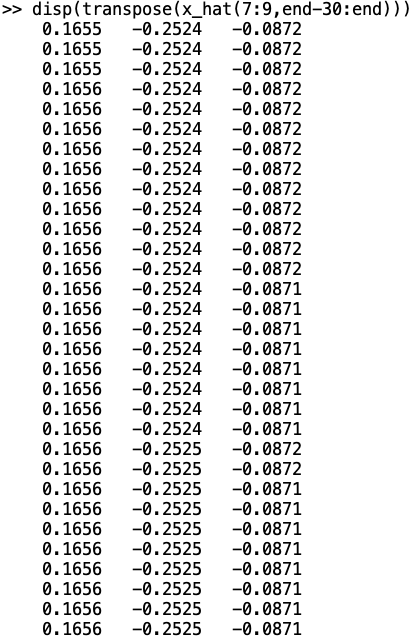
\includegraphics[width=1.6\linewidth]{EKF/AC_Bias.png}  
    \label{fig:Bias}
    \captionsetup{justification=centering} % Ensure caption is centered
    \captionof{figure}{Bias Convergence}
\end{minipage}\\

\textbf{If considering accelerometer bias is not a constant but gradually drifts over time, how will you modify the implementation of EKF to address this issue?}\\

1. The first step would be to augment the state vector to include the bias, which we have done currently.\\

2. The second step would be to model the bias dynamics assuming that it is a random walk, meaning that the bias would change over time with some associated process noise. For this, we would want to build a dynamic model as:
\begin{align*}
\mathbf{b}_{k+1} = \mathbf{b}_k + \mathbf{w}_b
\end{align*}
Where $w_b$ would be your process noise for bias.\\

3. The third step would be to update the measurement model by assuming that the accelerometer measurements are being affected by the true acceleration and the bias, making sure that the measurement model would account for the bias. This measurement model would be included in the H measurement matrix. Therefore if we denote the accelerometer measurement as $ac_k$, the model would become:
\begin{align*}
\mathbf{ac}_k = \mathbf{a}_k + \mathbf{b}_k + \mathbf{v}_k,
\end{align*}
where $a_k$ is the true acceleration of the UAV, $b_k$ is the accelerometer bias, and $v_k$ is the measurement noise.\\

4. The fourth step would be to tune the filter, since bias drift brings in additional uncertainty. Therefore we need to tune the process noise covariance (Q), such that if the noise for the bias is too low, then the filter would be too slow to adapt with the changes in bias, and if it is too high, then the filter could over correct to small noise fluctuations.\\

Implementing these 4 steps would help account for gradual drift in accelerometer bias, and would help modify the implementation of EKF to address these issues.

